\documentclass{scrartcl}
\usepackage[utf8]{inputenc} 
\usepackage[T1]{fontenc}
\usepackage{lmodern}
\usepackage[ngerman]{babel}
\usepackage{courier}
\usepackage{amsmath}
\usepackage{graphicx}
\usepackage{multicol}
\usepackage{geometry}
\usepackage{authblk}
\usepackage[font=scriptsize, labelfont=bf]{caption}
\usepackage{listings}
\usepackage{hyperref}
\usepackage{color}
\newenvironment{Figure}
  {\par\medskip\noindent\minipage{\linewidth}}
  {\endminipage\par\medskip}
  
\definecolor{dkgreen}{rgb}{0,0.6,0}
\definecolor{gray}{rgb}{0.5,0.5,0.5}
\definecolor{mauve}{rgb}{0.58,0,0.82}

\lstset{frame=tb,
  language=C,
  aboveskip=3mm,
  belowskip=3mm,
  showstringspaces=false,
  columns=flexible,
  basicstyle={\small\ttfamily},
  numbers=none,
  numberstyle=\tiny\color{gray},
  keywordstyle=\color{blue},
  commentstyle=\color{dkgreen},
  stringstyle=\color{mauve},
  breaklines=true,
  breakatwhitespace=true,
  tabsize=3
  }


% for skript letters like H...
\usepackage{mathrsfs}

\geometry{verbose,a4paper,tmargin=25mm,bmargin=25mm,lmargin=15mm,rmargin=20mm}

\title{Protokoll zum Versuch Nichtlineare Dynamik und Chaos}
\author{Nicolas Heimann, Jesse Hinrichsen}
\affil{\textit{Universität Hamburg}}
\date{2015}
\begin{document}
\maketitle




\begin{description}
\item Zusammenfassung
\end{description}


\section{  Einleitung  }
Alle Plottings und Simulationsn aus dem Versuch haben wir im Rahmen des Versuches selber implementiert. Dafür wählten wir als Programmiersprache Python2.7 und nutzten OpenGL4.1 und OpenCL für Berechnungen und Visualisierungen. Der Quellcode ist online über github einsehbar: \url{https://github.com/keksnicoh/gl_plotting_experimental}.  

Im folgenden bezeichnet $f^2(x) = f(f(x))$

\section{Logistische Abbildung}
Die logistische Abbildung ist gegeben durch $f(x_n)=x_{n+1}=rx_n(1-x_n)$. Es zeigt sich das diese einfache Funktionsvorschrift 
bereits chaotisches Verhalten an den Tag legt, welches wir im folgenden Abschnitt genauer untersucht haben. Zunächst haben 
wir ein Bifurkations Diagramm der logistischen Abbildung erzeugt indem wir den Parameter r gegen Iterationspunkte aufgetragen haben. Dabei fixierten wir jeweils ein r und erzeugten eine Folge $x_0 ... x_{1000}$ von welcher wir $x_{500} ... x_{1000}$ auf die y-Achse aufgetragen haben (Abbildung N).
Das Bifurkationsdiagramm lässt sich in mehrere Bereiche unterteilen. Bis $r=3$ haben laufen die $x_{500}...x_{1000}$ auf den gleichen Fixpunkt zu. An $r=3$ gabelt sich das Diagramm in zwei Äste aus (Periodenverdoppelung). An $r=3.449$ gibt es eine weitere Perdionenverdopplung und es ist eine Selbstähnlichkeit mit dem Bereich um $r=3$ zu erkennen (Fraktale Strukturen). Ab $r=3.569$ entsteht ein chaotischer Bereich in welchem sich aber noch Strutkuren feststellen lassen (Bögen, Punkte auf geraden, freie Bereiche).
\begin{figure}
	\centering
	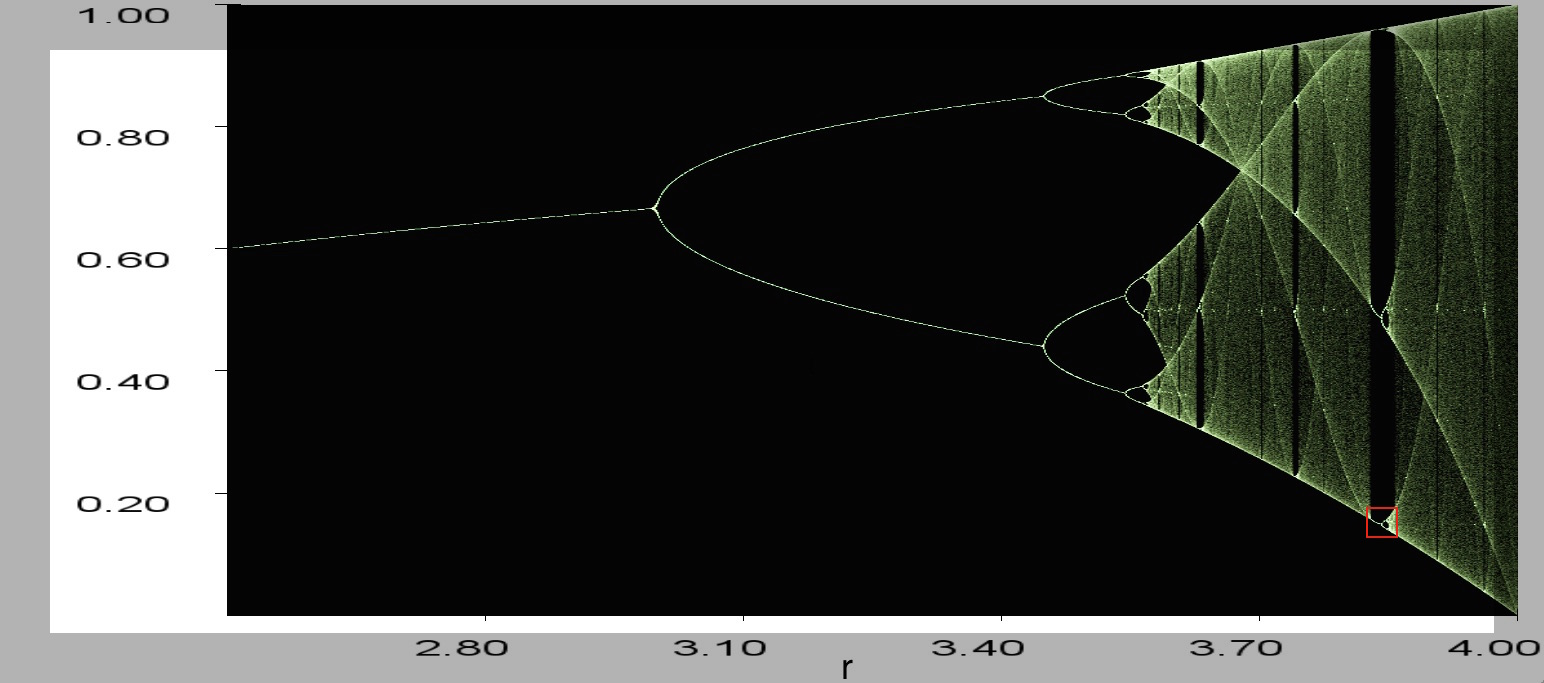
\includegraphics[scale=0.25]{bifurkation}
	\caption{Bifurkationsdiagramm der logistischen Abbildung im Bereich $r\in[2.6,4]$. sourcecode: prak/birukation-logistisch-no-opt.py}
	\label{bifurkation}
\end{figure}
\subsection{Fixpunkte / Stabilitätsbedigung}
Gilt für den Parameter $0 \textless r \textless 1$ dann konvergiert $f^n(x)$ gegen 0, denn $f^n(x)$ ist ein Polynom vom grad $2n$.
Bildet die Funktion einen Punkt idempotent ab, so handelt es sich um einen Fixpunkt, es gilt: $f^n(x^*)=x^* \forall n \iff x^* ist Fixpunkt$. 
Stabilitätsbedingung
$$|f'(x^*)|<1 \iff Fixpunkt-stabil$$
$$|f'(x^*)|>1 \iff Fixpunkt-instabil$$ Mit
\begin{math}
f(x^*)=rx^*(1-x^*)=x^*
\iff x^*=1-1/r \vee x'=0
\end{math}
ließ sich so analytisch bestimmen, dass die Fixpunkte für $r \in [0,1) \cup (3,4]$ instabil für $r \in (1,3)$ stabil sind.
Abbildung N zeigt das Verhalten der logisitschen Funktion für zwei solche Werte für r. So lässt sich auf die Aufspaltung im Bifurkationsdiagramm (Abblidung N) für $r>3$ verstehen. Abbildung N zeigt wie sich die Iteration jeweils für einen stabilen und einen Instabilen Wert von r verhält. 

\begin{figure}
\centering
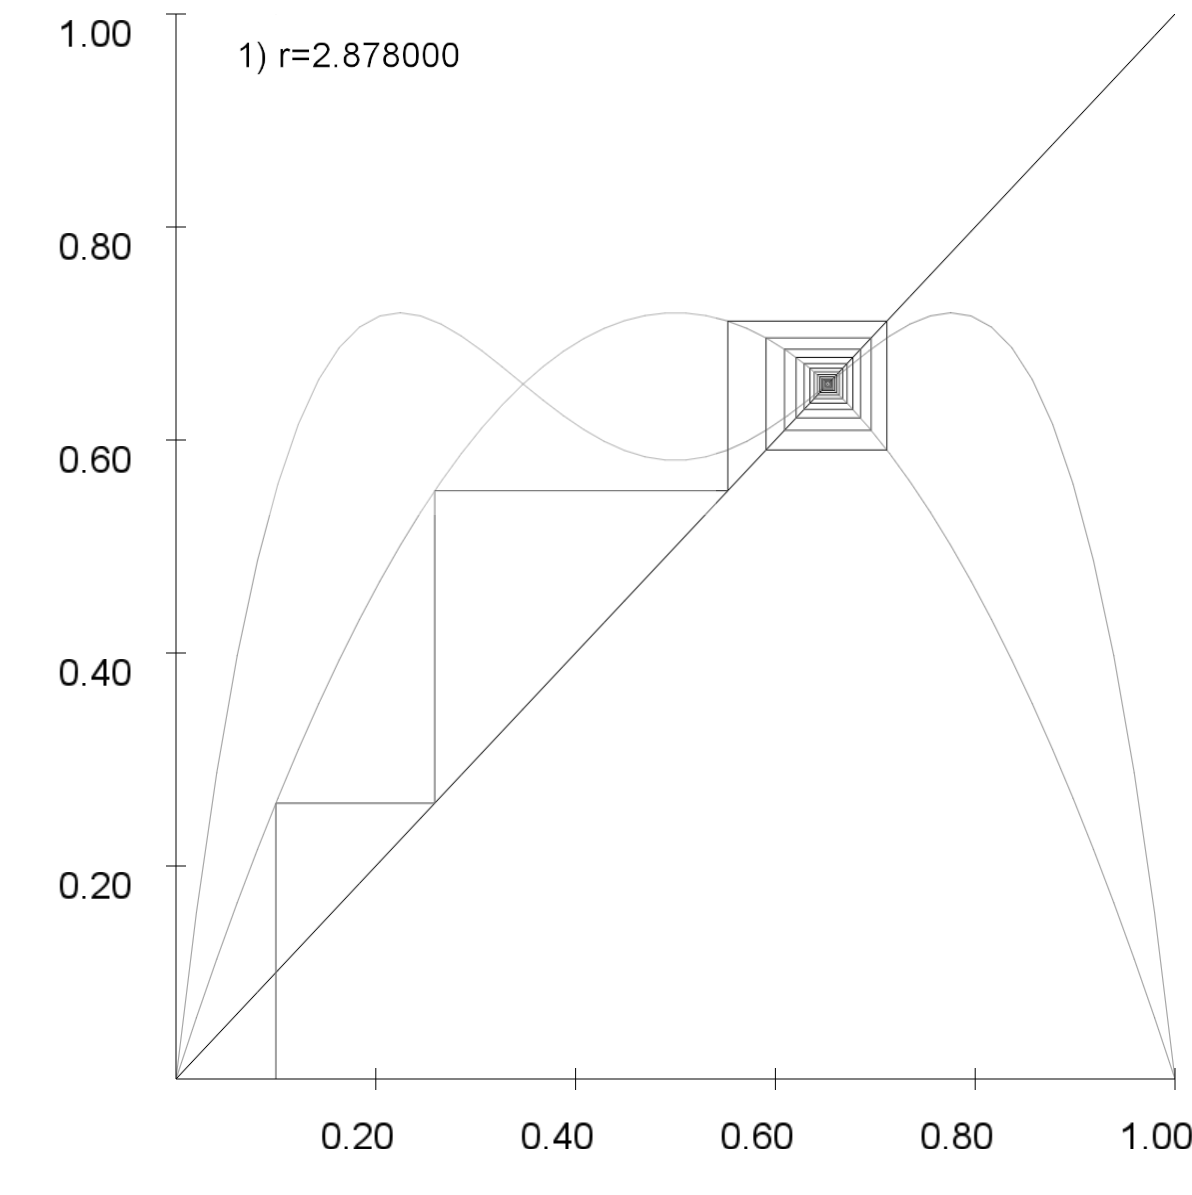
\includegraphics[scale=0.2]{fixpunkt-2878}
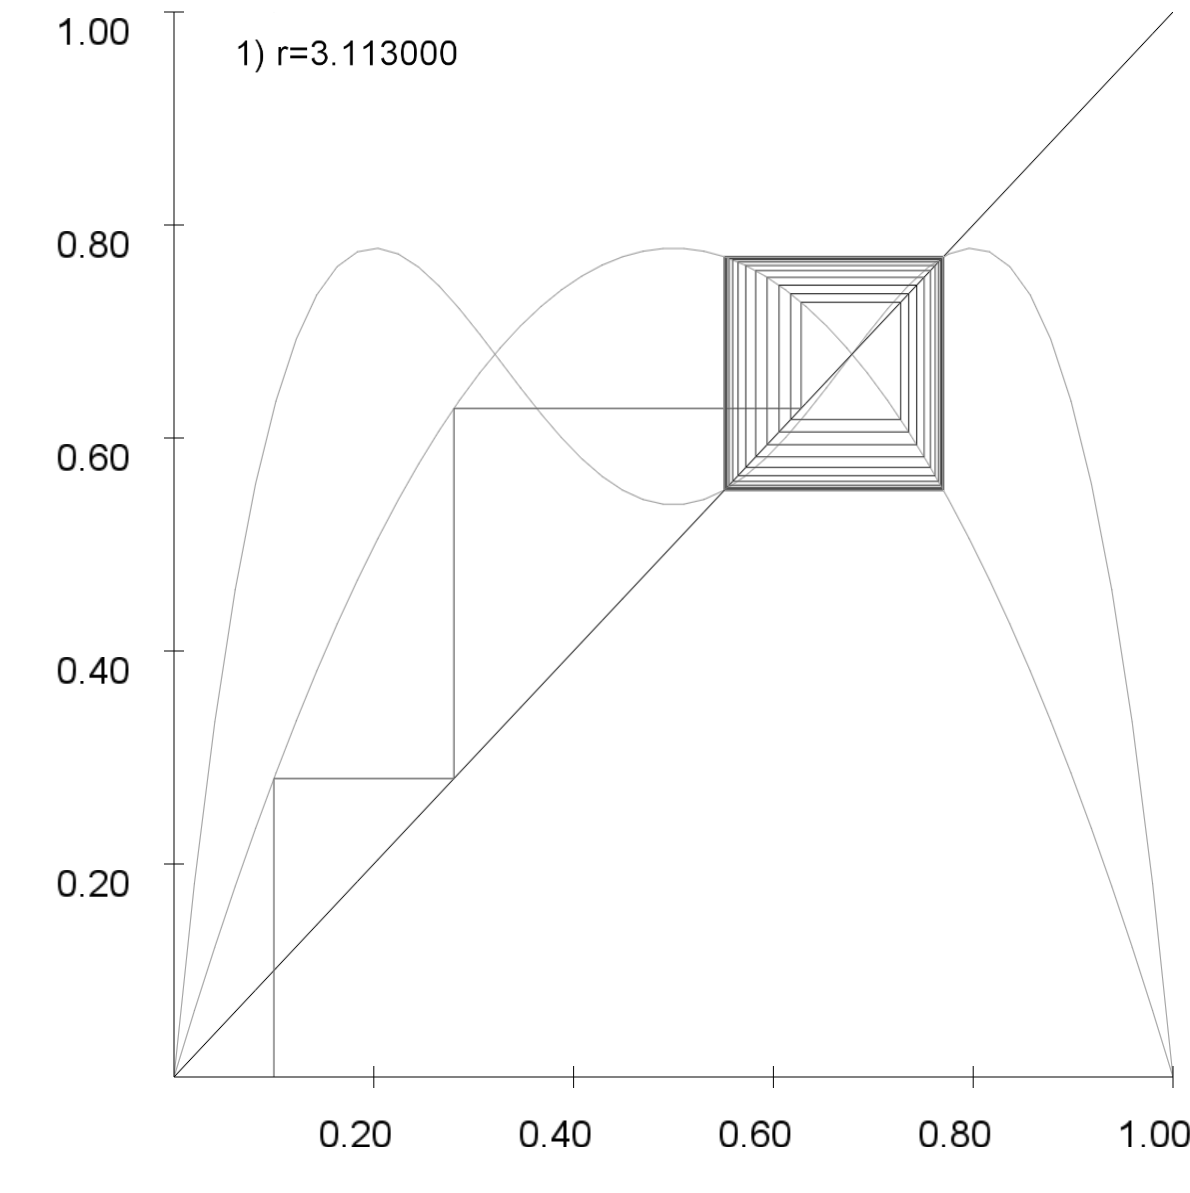
\includegraphics[scale=0.2]{fixpunkt-311}
\caption{Verlauf der Iterationen bei fixierten Parameter r. Linkes Bild zeigt einen Anziehenden Fixpunkt bei r=2.878, rechtes Bild zeigt abstroßenden Fixpunkt bei r=3.113. Der verlauf der logistischen Funktion $f(x)$ sowie $f^2(x)$ sind aufgetragen sowie die Einheitsgerade $y=x$. Als Linie Verbunden geplottet ist die Folge ($x_n, 0.0), (x_n, x_{n+1}), (x_{n+1}, x_{n+1}), (x_{n+1}, x_{n+2}), (x_{n+2}, x_{n+2}), (x_{n+2}, x_{n+3}), ...$ Sourcecode: prak/logisitsch-no-opt-behavior.py}. 
\end{figure}
\subsection{Lyapunov Exponent}
Der Lyapunov Exponent beschreibt mit welcher Geschwindigkeit sich zwei naheliegende Punkte voneinander entfernen. 
Es gibt drei Wege den Lyapunov Exponenten zu implementieren:

(1) Definition
$\lambda(x_0) = \lim_{N \rightarrow \infty}\lim_{\epsilon \rightarrow 0} \frac{1}{N}\log{\mid \frac{f^N(x_0+\epsilon)- f^N(x_0)}{\epsilon} \mid} $


(2) Analytisch
$\lambda(x_0) = \lim_{N \rightarrow \infty} \frac{1}{N} \sum_{i=0}^{N-1}  \log{f'(x)} $


(3) Renormiert:
$\lambda(x_0) = \lim_{N \rightarrow \infty} \frac{1}{N} \sum_{i=0}^{N-1}  \log{f'(x)} $


In Abbildung N haben wir die drei Möglichkeiten auf die logisitsche Funktion angewendet. Es zeigte sich, dass die erste Möglichkeit sehr schlechte Ergebnisse im Vergleich zu den beiden letzten Methoden ergibt. Dies liegt daran, dass die selbt bei kleinen EPSILON die Funktionswerte sehr schnell divergieren und somit die Definition des Differenzenquotienten keinen Sinn ergibt. 
Der Lyapunov Exponent hat seine Nullstellen dort wo die Abbildung ihre superattraktiven Stellen hat. Umgekehrt divergiert $\lambda(x_0)$ an den superattraktiven Stellen. Man erhält also Information über das Verhalten der Abbildung für bestimmte $x_0$. Tratsächlich kann man den Lyapunov-Exponenten über den mittleren Informationsverlust ausdrücken $\lambda(x_0)=-log(2)*\delta I$ (QUELLE). Im folgenden ist der OpenCL Quellcode der renomierten Formel des Lyapunov Exponenten.
Renomierte Formel implementiert als OpenGL Shader Kernel für die logistische Abbildung:
\begin{lstlisting}
float g(float r, float x) {
    return r * x * (1-x);
}
vec4 f(vec4 x) {
    float x0 = 0.4;
    float eps = 0.0001;
    float n = 10000;
    float summe = x0;
    for (int i=1; i < n; i++) {
        x0 = g(x.x, x0);
        summe += log(abs(g(x.x, x0+eps)-g(x.x, x0))/eps);
    }
    return vec4(x.x, summe/n, 0, 0.5);
}
\end{lstlisting}
 
\begin{figure}
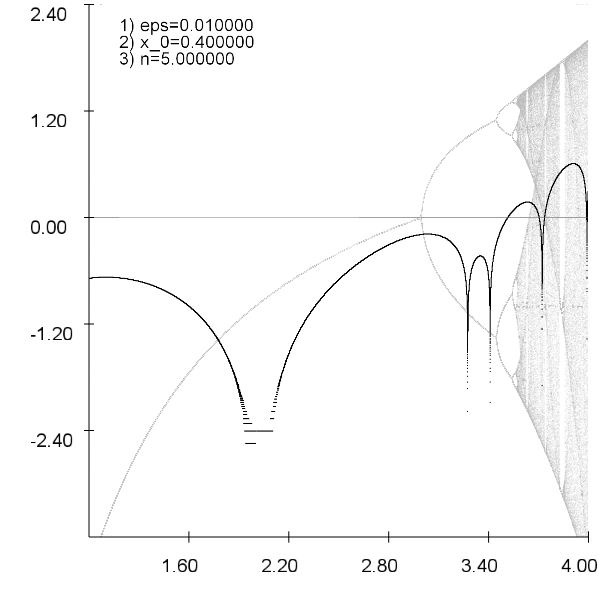
\includegraphics[scale=0.28]{iteration/lyapunov-1}
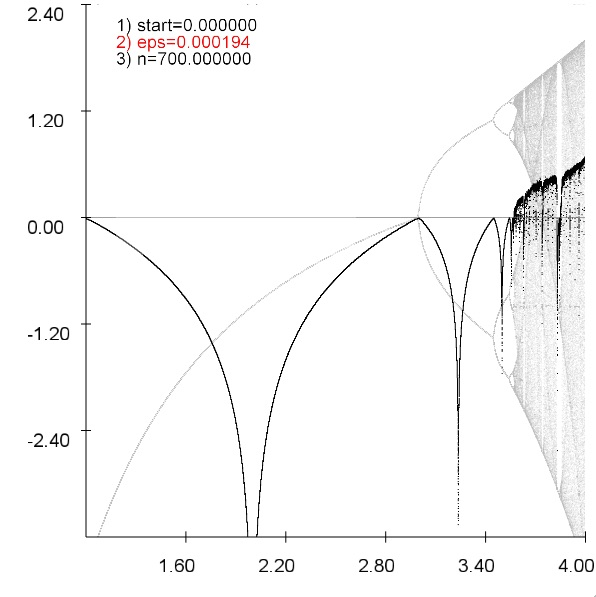
\includegraphics[scale=0.28]{iteration/lyapunov-2}
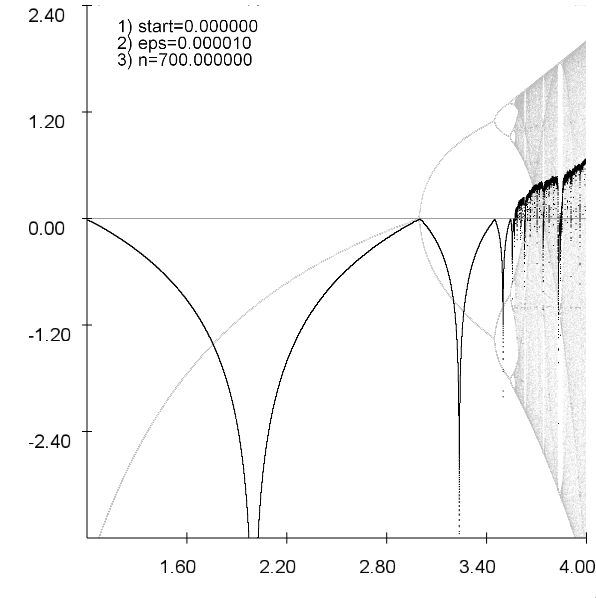
\includegraphics[scale=0.28]{iteration/lyapunov-3}
\caption{Die drei Lyapunov Exponent Implementation im Vergleich. Links: Definition, Mitte: Analytisch, Rechts: Renormiert. Die linke Implementation weißt deutliche Abweichungen im Vergleich zu den anderen beiden auf und ist somit unbrauchbar. Sourcecode: prak/lyapunov.py}. 
\end{figure}
\begin{figure}
\centering
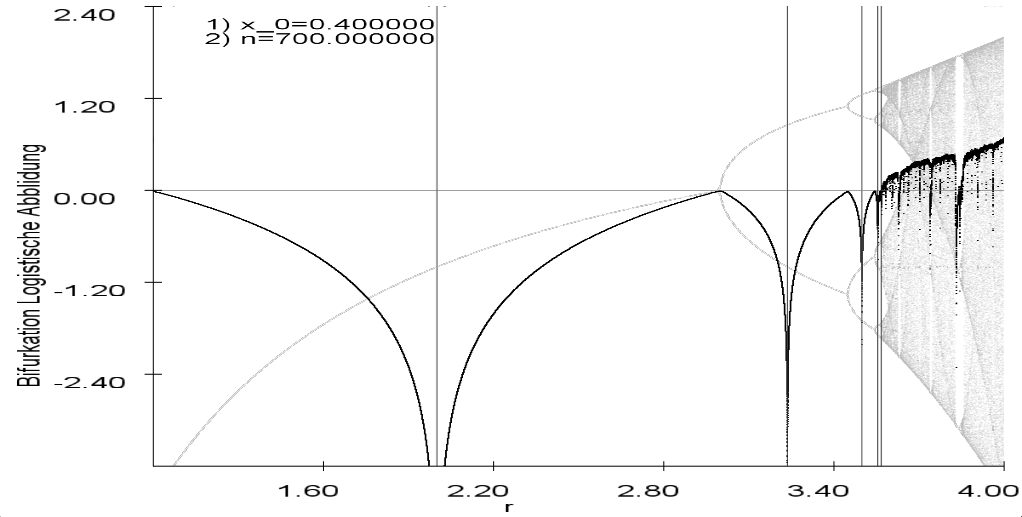
\includegraphics[scale=0.45]{iteration/bifurk-log-lyapunov-periode}
\caption{Analyse des Bifurkationsdiagrammes der logistischen Funktion. Eingezeichnet sind die y=0 Achse, sowie die ersten 5 Superattraktiven Stellen für r. Das Bifurkationsdiagramm wurde so translatiert und skaliert, dass es hinter dem Lyapunov Exponenten erscheint.}. 
\end{figure}


\section{Sinus Abbildung}
Die Sinusabbildung ist gegeben durch $x_{n+1}=r*sin(x)$. Wir haben die bereits implementieren Programme nun auf die Sinus Funktion angewendet und kamen zu folgendem Ergebniss:
 TABELLE MIT ALLEN SACHEN:

\begin{figure}
\centering
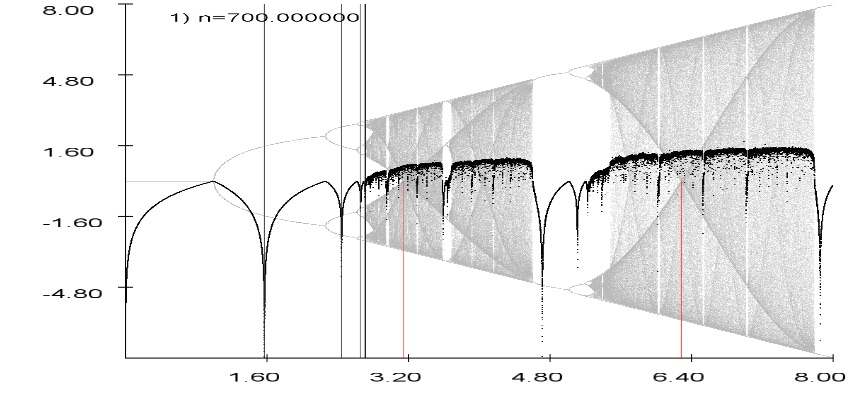
\includegraphics[scale=0.55]{bifurkation-sin}
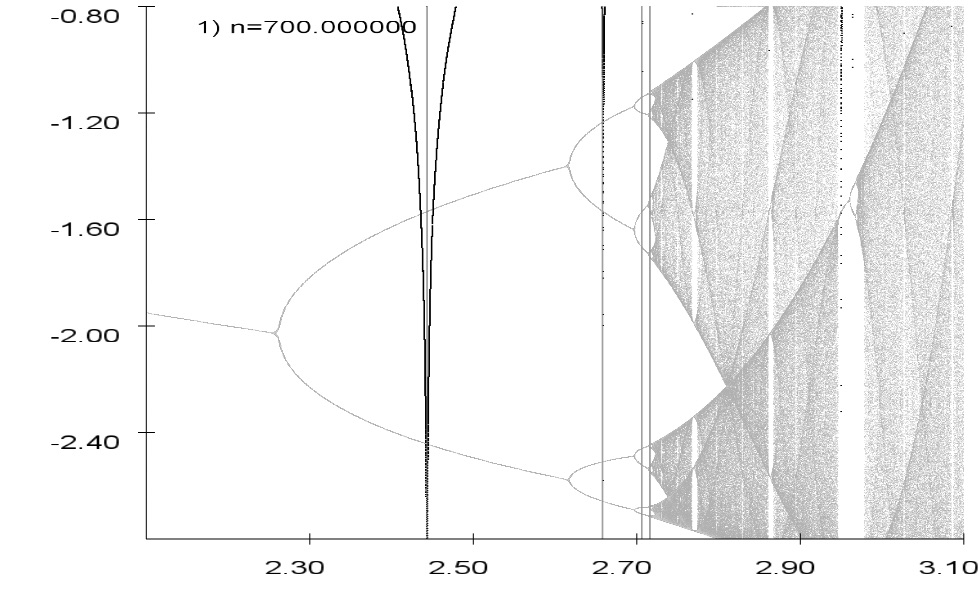
\includegraphics[scale=0.47]{bifurkation-sin-zoom}
\caption{Oben: Analyse des Bifurkationsdiagrammes der sinus Abbildung. Eingezeichnet sind die y=0 Achse, sowie die ersten 6 Superattraktiven Stellen für r (Erste Superattraktive Stelle bei $r=0$. Ebenfalls wurden $\pi$ und $2\pi$ eingezeichnet. Unten: Vergrößerung des Ausschnittes $r \in [2.1,3.1], y\in[-2.8,-0.8]$}. 
\end{figure}


\subsection{Feigenbaumkonstante}
Die Feigenbaumkonstante ist eine universelle Größe. Sie tritt in chaotischen nicht linearen System auf und lässt sich wie folgt bestimmen:
$$\delta_i = \frac{b_i-b_{i+1}}{b_{i+1}-b_{i+2}}$$ oder $$\delta_i = \frac{s_i-s_{i+1}}{s_{i+1}-s_{i+2}}$$
$$\lim\limits_{i \rightarrow \infty}{\delta_i} = 4.669201609102991 (2.3.1) $$ (https://oeis.org/A006890)
wobei $s_i, b_i$ die Folgen der superattraktiven und periodenverdoppelden Stellen sind.
Also lässt sich die Feigenbaumkonstante mit dem Lyapunov Exponenten bestimmen. 
Wir haben uns dazu entschieden, die superattraktiven Fälle numerisch zu finden, da diese leichter zu ermitteln sind (Infimum). Die Nullstellen sind bei genauerem hingucken nicht präzise weshalb ein sehr schwammiges Epsilon Kriterium die Genauigkeit verwischt hätte (Siehe Abbildung N XXX). 
Der Algorithmus startet im Suchmodus bei gegeben Startwert $x_{start}$ und geht in kleinen Schritten $\Delta x$ die x-Achse ab. In jedem Schritt wird $l_1=\lambda(x_0)$ $l_2=\lambda(x_0 + \Delta x)$ berechnet. 
Ist $l_2-l_1 \leq 0$ $(1) $ wandert der Iterationsschritt zum superattraktiven Fall. 
Dies wird so lange fortgesetzt bis die Bedingung $(1)$ nicht mehr hält. 
Es wird nun um $\Delta x$ zurueckgegangen und anschließend die Schrittweite $\Delta x \mapsto \frac{\Delta x}{10} $ verkleinert. Nun wird erneut so lange iteriert, bis $(1)$ nicht mehr hält. 
Der Vorgang wiederholt sich 8 mal. Nun wird $(2*x_0 + \Delta x )/2$ als Ergebniss gespeichert. 
Als nächstes befindet sich der Algorithmus im Anfangspunkt-Modus. Es wird so lange die x-Achse abgetestet bis die Bedingung $\lambda(x_0) < \lambda(x_0 + \Delta x) < \lambda(x_0 + 2*\Delta x)$ nicht mehr erfuellt ist und somit ein neues $x_{start}$ gefunden wurde. Der Suchmodus wird aktiviert.  (Quellcode: prak/feigenbaum.py)
Im folgenden ist die Terminal Ausgabe des Algorithmusses beigefuegt:
\begin{lstlisting}
searching from 1.9
looking for next start_r from 2.00000000002
searching from 2.99950000003
looking for next start_r from 3.23606797751
searching from 3.44927797752
looking for next start_r from 3.49856169934
searching from 3.54400769935
looking for next start_r from 3.55464086278
searching from 3.56439786279
looking for next start_r from 3.56666737986
found values [2.0000000000249916, 3.236067977509959, 3.498561699344952, 3.554640862779951, 3.5666673798649517]
delta_0=4.70894301336
delta_1=4.68077099865
delta_2=4.66295961155
\end{lstlisting}
Somit konnten wir für $n=2$ eine Feigenbaumkonstante von $\delta_2=4.66295961155$ numerisch berechnen. Dieser Wert weicht um 0.133671789\% vom tatsächlichen Wert (2.3.1) ab. $$x_{n+1}=f_r(x_n)=rx_n(1-x_n)$$
$$\Rightarrow x_{n+2}=r^2x_n(1-x_n)(1-rx_n(1-x_n))$$
\newline
Fixpunktgleichung (Einerzyklus): 
$$x=rx(1-x)$$
$$\Rightarrow x_1=0, x_2=1-\frac{1}{r}$$
Startwerte x=0 und x=1 haben den Fixpunkt $x_1$ wohingegen für alle $x\in (0,1)$ der Fixpunkt $x_2$ ist.
\newline
Fixpunktgleichung (Zweierzyklus):
$$x=r^2x(1-x)(1-rx(1-x))$$
$$\Rightarrow x_{3,4}=\pm\frac{\sqrt{r^2-2 r-3}+r+1}{2 r}$$
Damit $x_{3,4}$ reel bleibt muss $r^2-2 r-3 \geq 0$
$$\Rightarrow r \leq -1 \land r \geq 3$$
Für diesen Bereich gibt es folglich 2 weitere Fixpunkte $x_{3,4} \Leftrightarrow$ Perdiodenverdopplung 
\newline
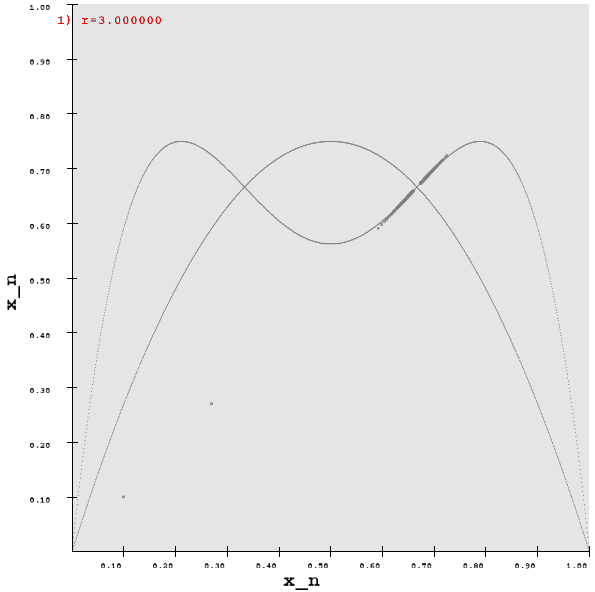
\includegraphics[scale=0.3]{r3}
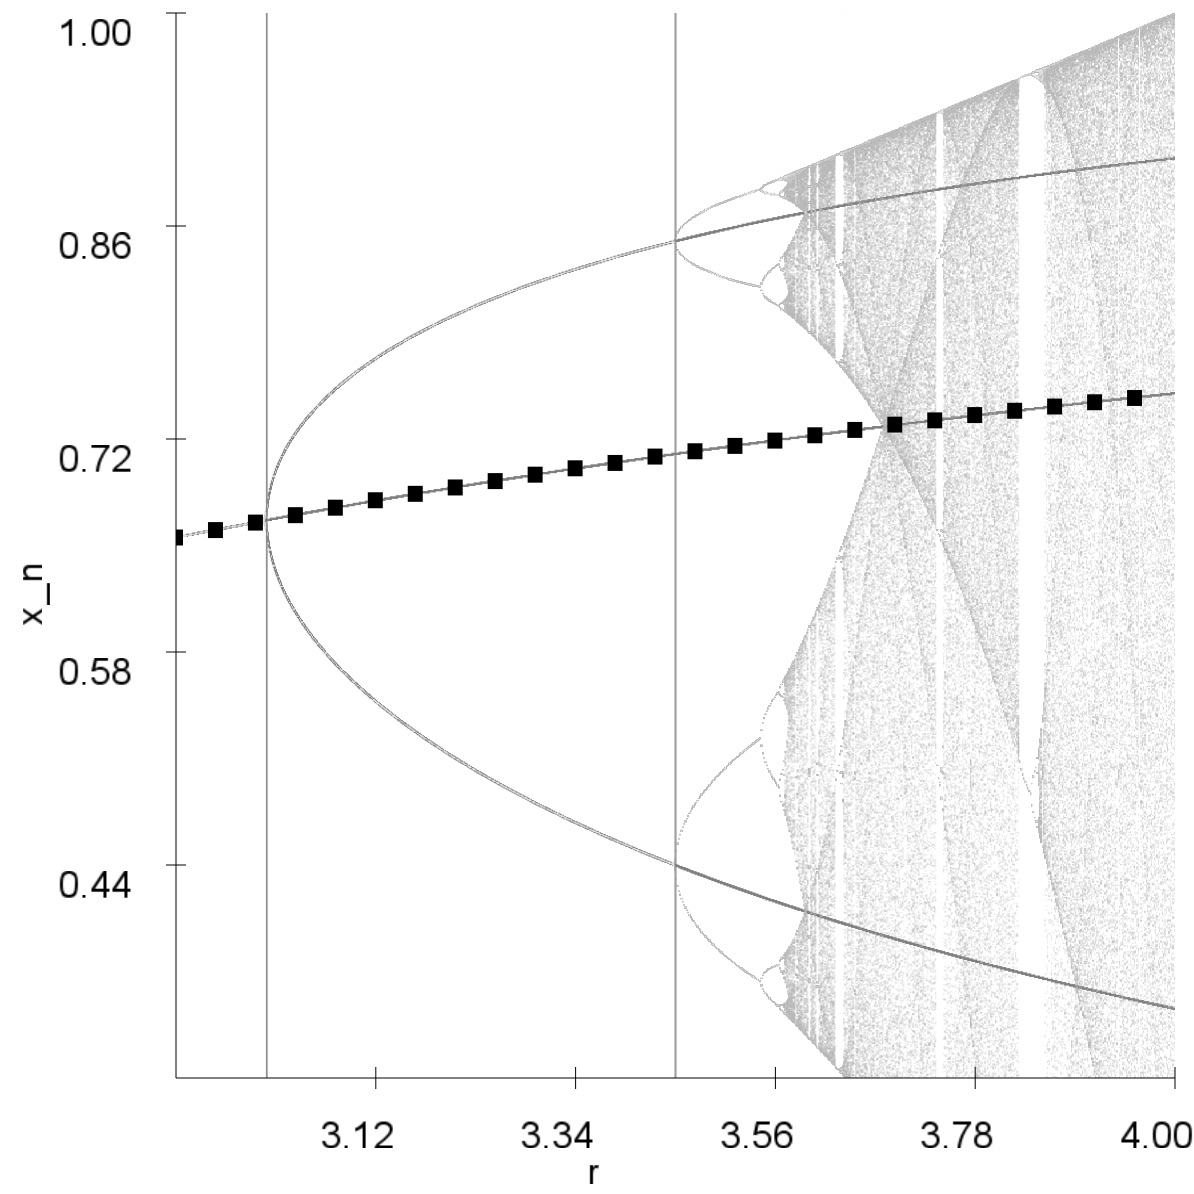
\includegraphics[scale=0.3]{analy-periodenv}
\newline
\subsection{ Stabilitätsbedingung }
Ein Fixpunkt ist stabil, wenn gilt:
$$\mid f'(x)\mid <1$$
Im Fall der logistischen Abbildung gilt
$$\frac{d}{dx}f(x)=r-2rx=r(1-2x)$$
$$\frac{d}{dx}f^2(x)=-r^2(2x-1)(2r(x-1)x+1)$$
\newline
Es gilt zu lösen, für welche $r$ bei bekannten Fixpunkte die Stabilitätsbedingung erfüllt ist.
\newline
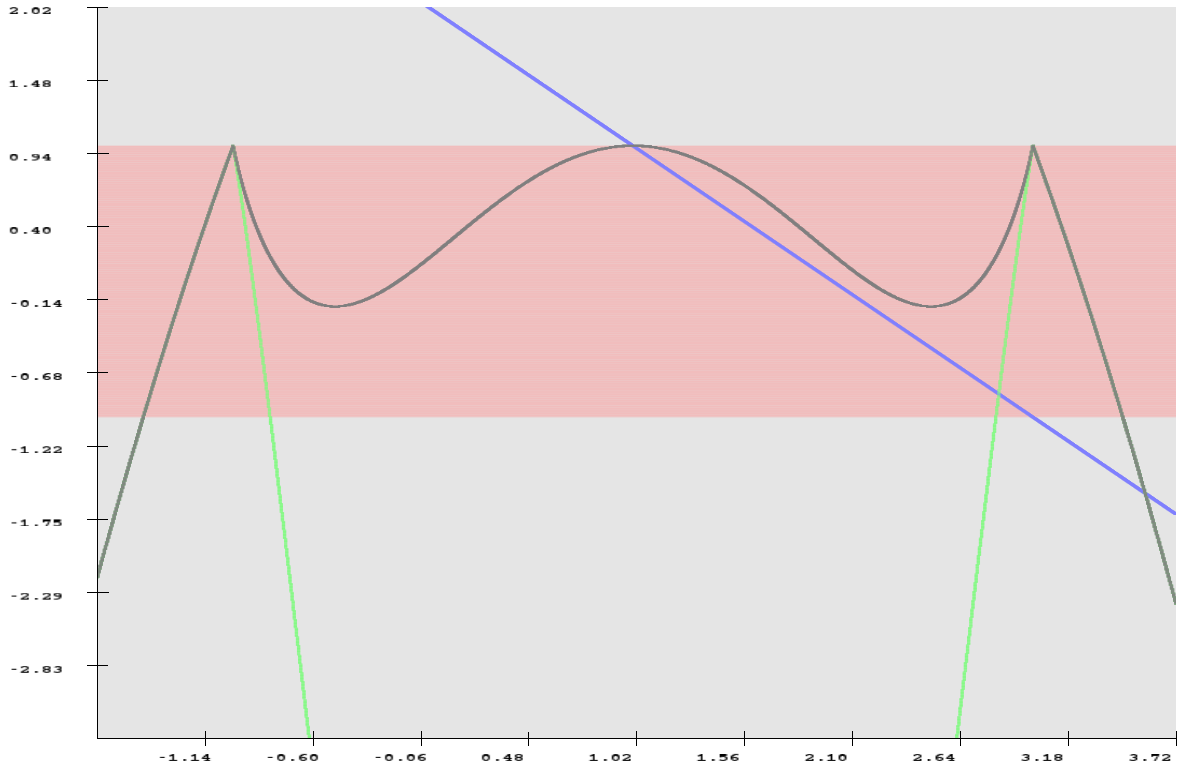
\includegraphics[scale=0.4]{stable_fixpoints}
\newline
Grafisch lässt sich ablesen, dass der Fixpunkt $x_3=\frac{\sqrt{r^2-2 r-3}+r+1}{2 r}$ (grüner Graph) für folgende Bereiche stabil ist:
$$-1.45<r<-0.82 \Rightarrow -1.45 < r \leq -1$$
$$2.82<r<3.45 \Rightarrow 3 \geq r > 3.45$$
Der Fixpunkt $x_4=\frac{-\sqrt{r^2-2 r-3}+r+1}{2 r}$ (grauer Graph) ist im gesamten Bereich $-1.45<r<3.45$ stabil aber da der Fixpunkt ebenfalls nur für $r \leq -1 \land r \geq 3$ existiert gilt der selbe Bereich wie für $x_3$. Die Fixpunkt sind dort stabil, wo sich der graue und der grüne Graph in der Abbildung überlagern.
\section { Bifurctationsdiagramm}
\subsection { Logistische Abbildung }
asdf
\subsection { Sinus Abbildung }
asdf
\section{ Feigenbaumkonstante}
\subsection {Lyapunov}
Eine Möglichkeit die Feigenbaumkonstante zu berechnen ist über die Nullstellen des Lyapunov-Exponenten. Gerade an diesen Stellen kommt es zu einer Periodenverdopplung. Dann lässt sich die Feigenbaumkonstante durch
$$\delta = \lim_{n \rightarrow \infty}\frac{a_{n-1}-a_{n-2}}{a_n-a_{n-1}}$$
, wobei die $a_n$ der Parameter ist bei dem die n-te Periodenverdopplung auftritt.
\newline
Für dern Lyapunov-Exponenten gilt:
$$\lambda(x_0) = \lim_{N \rightarrow \infty}\lim_{\epsilon \rightarrow 0} \frac{1}{N}\log{\mid \frac{f^N(x_0+\epsilon)- f^N(x_0)}{\epsilon} \mid} $$
oder auch
$$\lambda(x_0) = \lim_{N \rightarrow \infty} \frac{1}{N} \sum_{i=0}^{N-1}  \log{f'(x)} $$

\begin{figure}
	\centering
	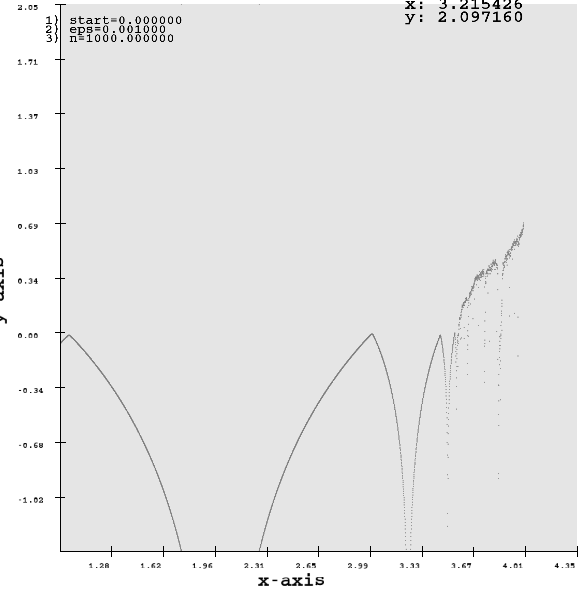
\includegraphics[scale=0.65]{lyapunov_1000}
	\caption{Lyapunov mit N=1000 und $\epsilon=0.001$ (Logistische Abbildung). Parameter r auf der x-achse und $\lambda(x_0)$ auf y-achse, mit startwert $x_0=0.4$}
	\label{img:lyapunov_100}
\end{figure}
Wie erwartet ist eine Nullstelle bei $x=3$. Gucken wir uns allerdings den Bereich für $x=3$ genauer an, so stellen wir eine gewisse Ungenauigkeit fest (vgl. nächste Abbildung). Da wir für die Feigenbaumkonstante möglichst genau die Stellen an denen Periodenverdopplung auftritt identifizieren wollen, müssen wir die Parameter entsprechend modifizieren. Die Fluktuation nehmen zu, wenn $\epsilon$ kleiner wird.
\begin{figure}
	\centering
	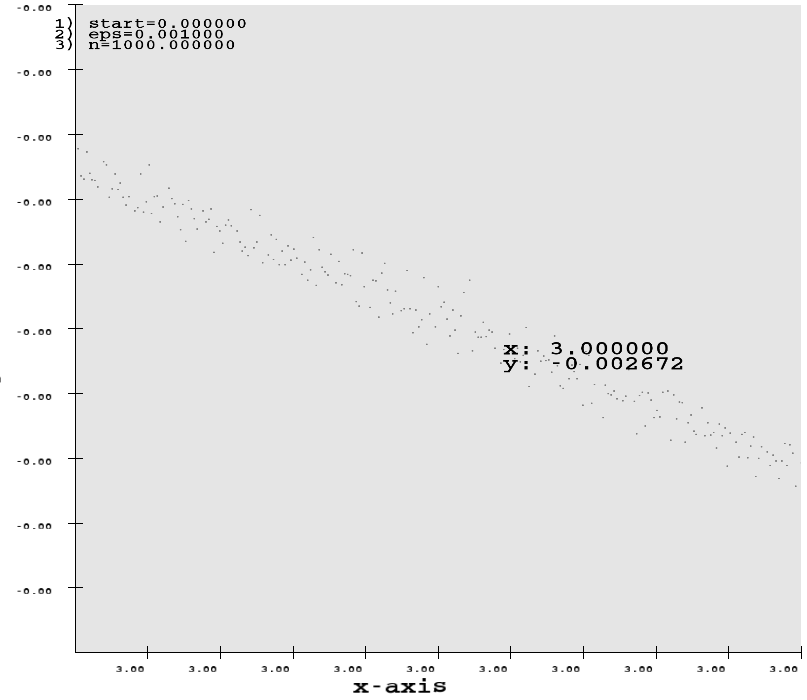
\includegraphics[scale=0.50]{lyapunov_1000_at_3}
	\caption{1. Bei $x=3$ erhalten wir einen von 0 verschiedenen Wert ($\lambda\approx-0,0027$) 2. Wie stellen fest das der Lyapunov-Exponent für unterschiedliche r fluktuiert.}
	\label{img:lyapunov_1000_at_3}
\end{figure}
\newline
@TODO: Bei N -> 13000 und epsilon < 0.00001 kommt man schon ganz gut dran!
1. Verhalten wenn man erst später anfängt zu summieren
2. Bei gegebener Konfiguration für r=3 messen mit Fehler etc.
3. Weitere Periodenverdopplungen grafisch identifizieren. (Domain hoch setzen für bessere Genauigkeit)
4. Ursache für Fluktuationen?? Und Möglichkeit diese Fluktuationen zu mitteln!?
5. Mit gemittelter Fluktuation in OpenCL nicht-grafisch Nullstellen identifiezieren (double precision!!! -> Fehler der durch float64 berücksichtigt werden muss)

\section { Duffing-Gleichung}
Wir betrachten nun ein angetrieben und gedämpften Oszillator. Als Unterschied zum klassischen Harmonischen Oszillator wird der Term mit der Federkonstante kubisch.
$$\ddot{x}+\lambda\dot{x}+\beta x^3=\epsilon\cos{\Omega t}$$
Diese DGL lässt sich nun nicht mehr analytisch berechnen.
Im Folgenden lösen wir die Gleichung mit der Euler-Methode als auch mit dem Runge-Kutta Verfahren.
$$\frac{dy}{dt}=\epsilon\cos{\theta}-\lambda y - \beta x^3$$
$$\frac{dx}{dt}=y$$
$$\frac{d\theta}{dt}=\Omega$$
\subsection { Attraktoren }
Parameter:
$$\epsilon = 0,2, \lambda = 0,08, \beta = 1, \Omega = 1$$
- Unterschiede Runge Kutta Euler (unterschiedliche attraktoren)
\newline
- stabile / instabile Trajektorien --> parameter $h = \frac{Zeit}{Iterationen}$
\newline
- Optimierung durch Schrittweiten adaptierung
\newline
- lyapunov??
\subsection{ Poincareschnitt }
Die gezeigten Phasenraumportaits sind projektionen des dreidimensionalen Phasenraums $(x,y,\theta)$ auf die $(x,y)$ Ebene. Der Poincaree Schnitt ist eine Abbildung aller $(x,y)$ welche eine Ebene im Phasenraum schneiden. In Abbildung XYZ ist ein Bereich Poincaree Schnitt des Duffing-Oszillators mit $\epsilon=7.72$ und $\theta=0$ gezeigt. Zur Implementation des Poincaree Schnittes wählten wir $\theta=0$ um die Praktikumsanleitung als Test unserer Software nutzen zu können. Dabei nutzten wir $sin(\theta_1)*sin(\theta_2) \leq 0.0 \iff Ebenenschnitt$:
\begin{lstlisting}
      pos = sin(theta);
      if (last_pos*pos <= 0.0f) {
          result[k*2] = last_x;
          result[k*2+1] = last_y;
          k++;
      }
      last_pos = pos;

\end{lstlisting}
Dieses Verfahren zeigt bei genauerer Betrachtung aber leichter Ungenauigkeiten. So wird nicht exakt das $(x,y)$ duplet abgebildet bei welchen die Ebene geschnitten wurden, stattdessen wird das $(x,y)$ Duplet bei $\theta_2$ angezeit. Eine Möglichkeit dies zu Optimieren wäre den Mittelwert $(\frac{x_1+x_2}{2}, \frac{y_1 + y_2}{2})$ als Schnittpunkt zu identifizieren.
\begin{figure}
	\centering
	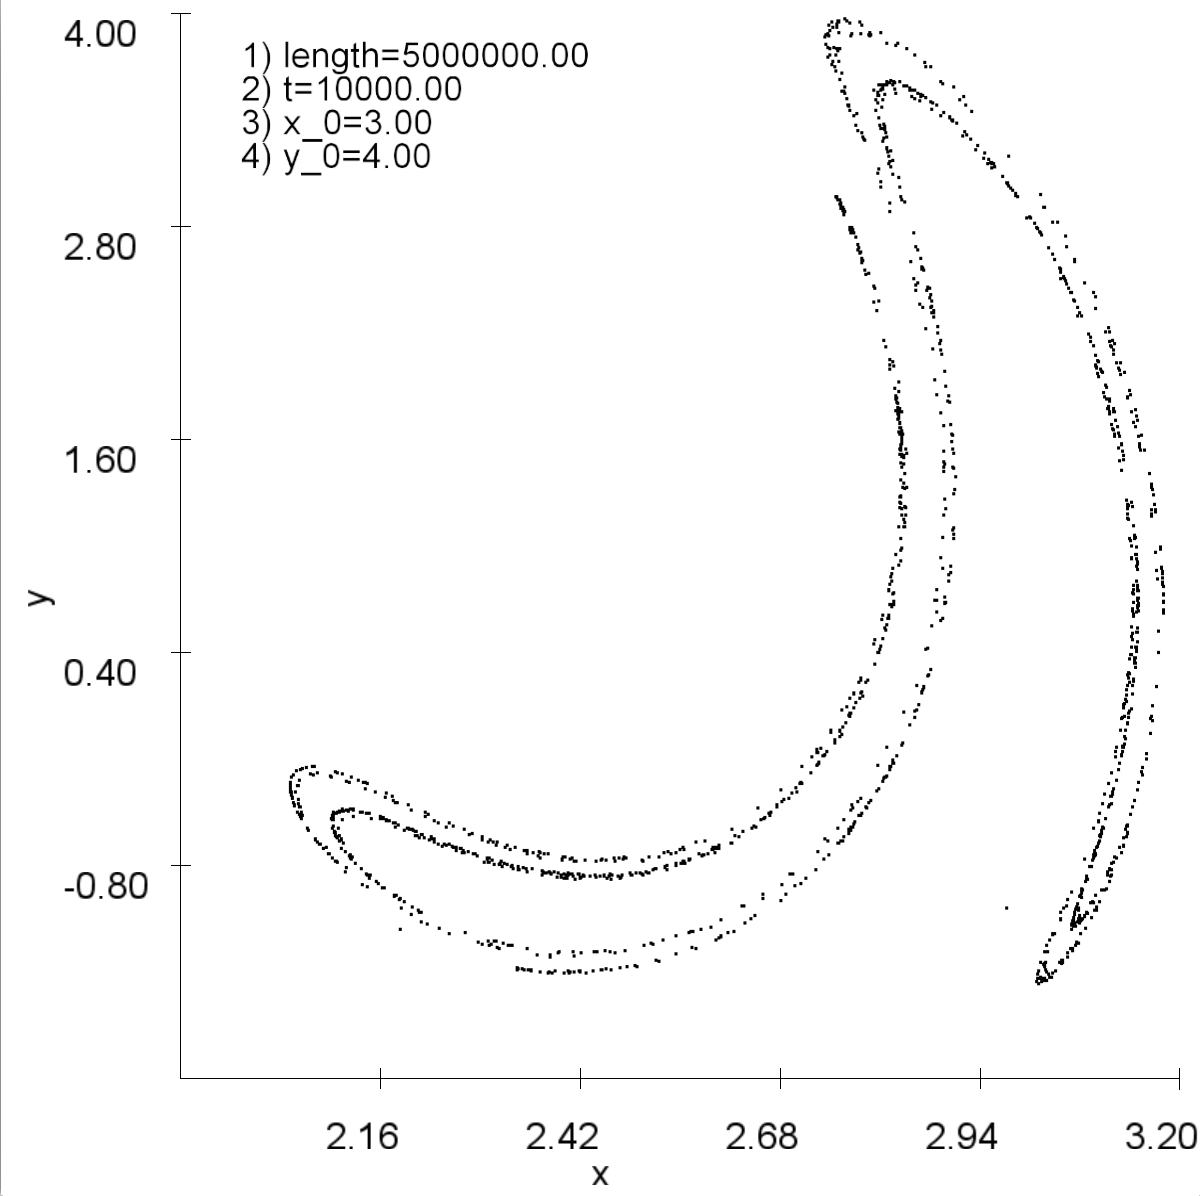
\includegraphics[scale=0.20]{poincare-772}
	\caption{Poincare Schnitt des Duffing Oszillators für $\epsilon=7.72 x=3.0, y=4.0, \lambda=0.2, \beta=1, \theta=1$. als Referenz aus dem VORBEREITUNGSHEFT-LITERATUR-S38}
	\label{img:poincare-772}
\end{figure}
\section {LDR-Oszillator}



\begin{figure}
	\centering
	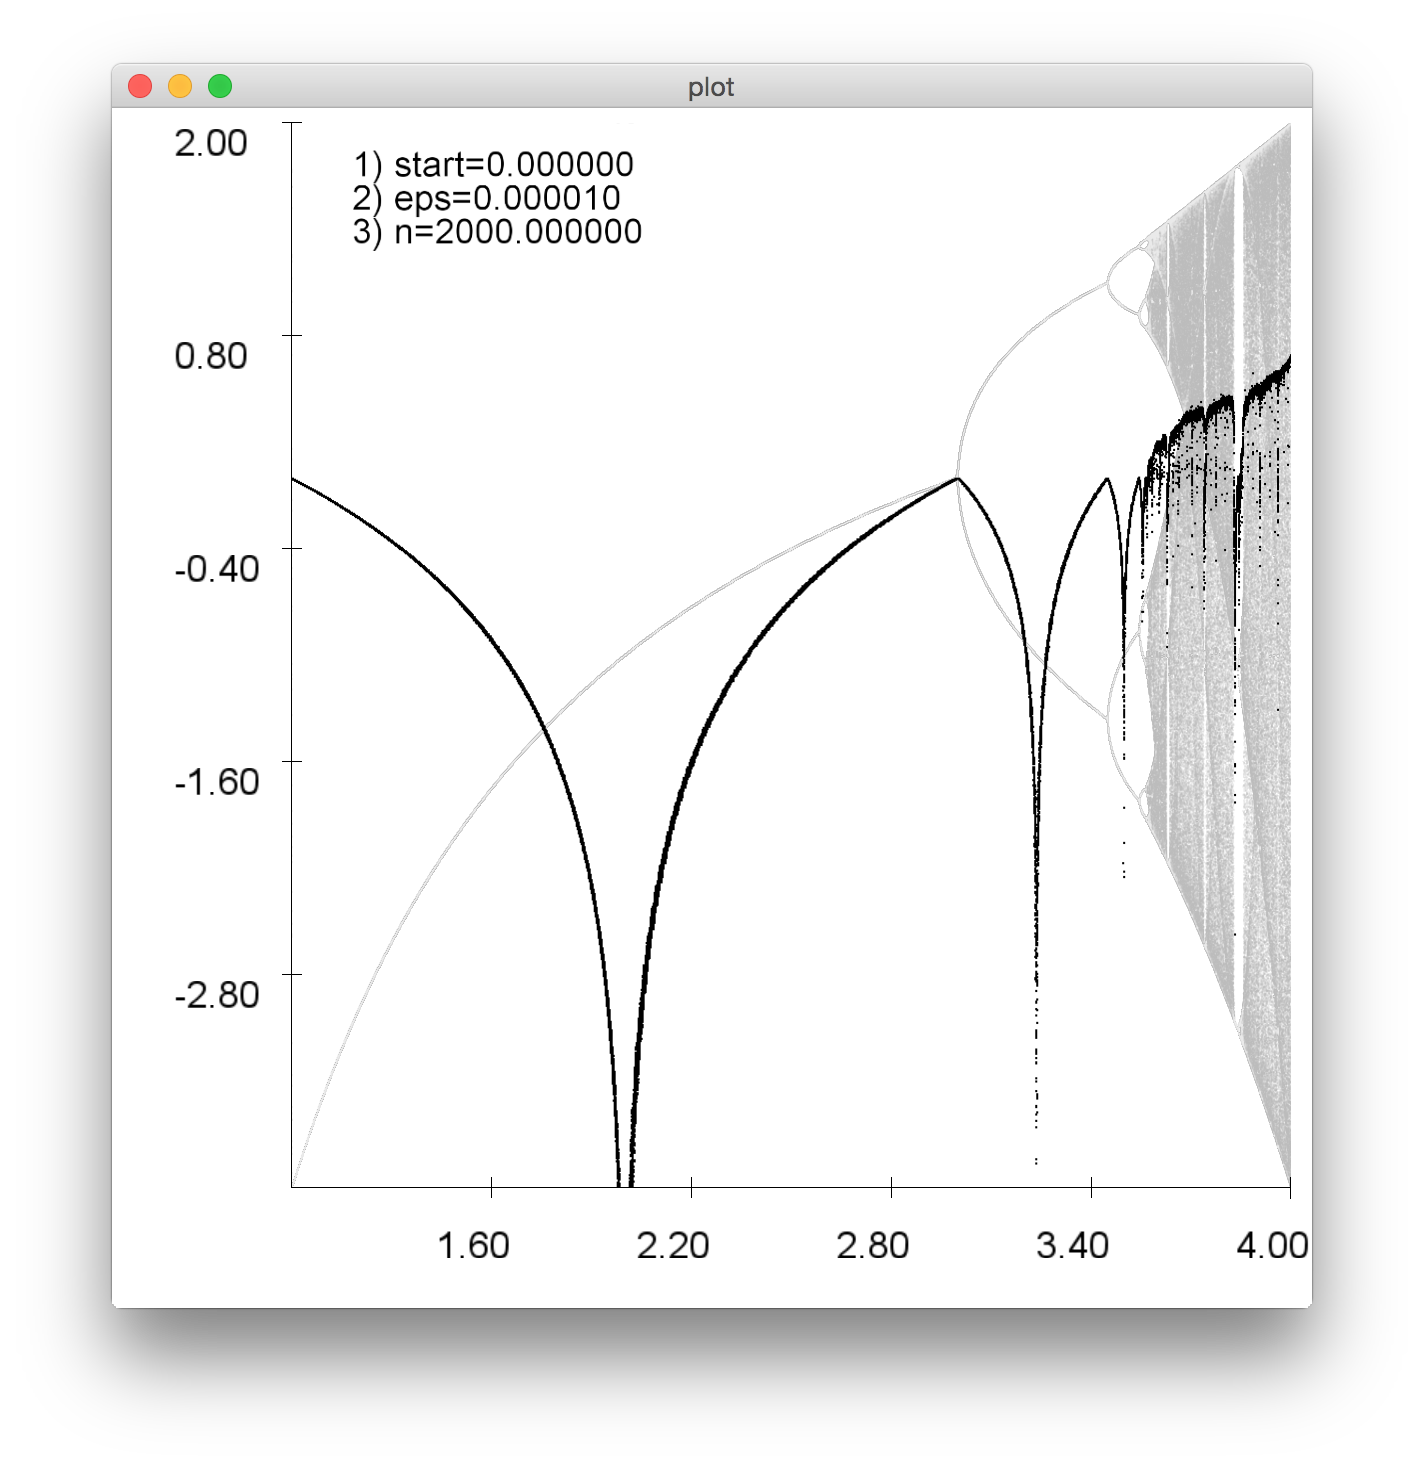
\includegraphics[scale=0.60]{lyapunov-log}
	\caption{asdf}
	\label{img:lyapunov-log}
\end{figure}
\section {LDR-Oszillator}


\section{ Literatur }
\begin{itemize} 
\item Nichtlineare Dynamik und Chaos - Physikalisches Praktikum für Fortgeschrittene Universität Hamburg
\end{itemize}




\end{document}







